\newcommand{\plasfig}{
  \def\height{128bp}
  \centering
  \tikzsetnextfilename{effect_of_plas}
  \resizebox{0.5\linewidth}{!}{
    \begin{tikzpicture}[
        >=stealth',
        overlay/.style={
            anchor=south west,
            draw=black,
            rectangle,
            line width=0.8pt,
            outer sep=0,
            inner sep=0,
          },
      ]
      \matrix[
        matrix of nodes,
        column sep=2pt,
        row sep=0pt,
        ampersand replacement=\&,
        inner sep=0,
        outer sep=0
      ] (pictures) {
        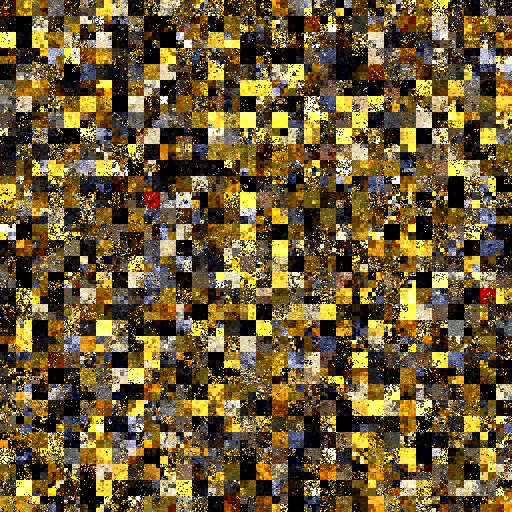
\includegraphics[height=\height]{assets/\clogdirname/plas/unsorted_colors.png} \&
        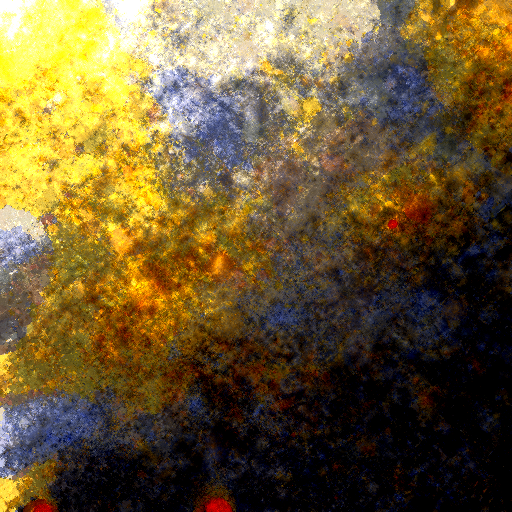
\includegraphics[height=\height]{assets/\clogdirname/plas/sorted_colors.png} \\
      };
      \node[above=0.4em of pictures-1-1.north, anchor=base] {Without PLAS};
      \node[above=0.4em of pictures-1-2.north, anchor=base] {With PLAS};
    \end{tikzpicture}
  }
}
\begin{figure}[t]
  \centering
  % \includegraphics[width=\linewidth, height=5em]{example-image-a}
  \plasfig
  \caption{\textbf{Effect of using PLAS~\cite{morgenstern2024compact} --}
    We demonstrate the effect of sorting by visualizing the decoded Gaussian
    colors in the UV map, for the \texttt{lego} sequence from the NeRF
    Synthetic~\cite{mildenhall2020nerf} dataset.
    After sorting, the UV map has smoother color transitions, confirming the
    successful spatial clustering of similar Gaussians.
  }
  \label{fig:clog-effect-of-plas}
\end{figure}